\documentclass[10pt]{beamer}
\usepackage[T1]{fontenc}
\usepackage[utf8]{inputenc}
\usepackage[english]{babel}
\usepackage{amsmath,pgfplots}
\usetheme{Copenhagen}
\usecolortheme{beaver}
\setbeamertemplate{navigation symbols}{}
\pgfplotsset{compat=1.18}
\title{Quadratic Functions and Vertical Motion}
\author{Cesare Peli}
\date{}
\begin{document}
\frame{\titlepage}
\begin{frame}{The Physical Model}
\begin{block}{Assumptions}
Treat the ball as a point mass, neglect air resistance, and take gravitational acceleration \(g\) as constant. Choose height positive upward. Initial height and vertical velocity are \(s_0\) and \(v_0\).
\end{block}
\[
h(t)=s_0+v_0t-\frac12gt^2,
\qquad v(t)=v_0-gt.
\]
This approximation describes motion close to the Earth's surface over a range in which variations of \(g\) are negligible.
\end{frame}
\begin{frame}{Quadratic Form and Maximum Height}
\begin{block}{The Vertex}
For \(y=ax^2+bx+c\), with \(a\ne0\), the vertex is at \(x=-b/(2a)\). In vertical motion,
\[
a=-g/2,\qquad b=v_0,\qquad c=s_0.
\]
For an upward launch, \(v_0>0\), the maximum occurs at
\[
t_{\max}=v_0/g,\qquad h_{\max}=s_0+v_0^2/(2g).
\]
At this time \(v=0\), and the negative quadratic coefficient makes the stationary point a maximum.
\end{block}
\end{frame}
\begin{frame}{Calculated Trajectory}
\begin{center}
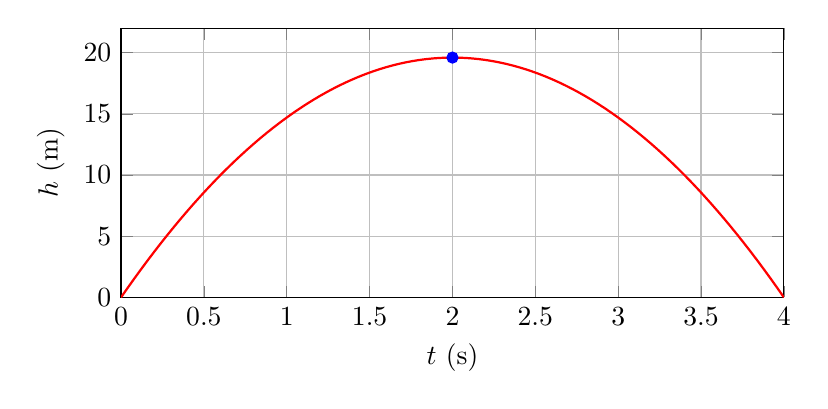
\begin{tikzpicture}
\begin{axis}[width=10cm,height=5cm,xlabel={\(t\) (s)},ylabel={\(h\) (m)},xmin=0,xmax=4,ymin=0,ymax=22,grid=major]
\addplot[red,thick,domain=0:4,samples=101] {19.6*x-4.9*x*x};
\addplot[only marks,mark=*,blue] coordinates {(2,19.6)};
\end{axis}
\end{tikzpicture}
\end{center}
\small The curve is calculated from \(h(t)=19.6t-4.9t^2\). The modeled ball returns to ground level at \(t=4\) s.
\end{frame}
\begin{frame}{Exercise}
A ball is launched vertically from ground level with initial speed \(v_0=19.6\) m/s. Neglect air resistance and use \(g=9.8\) m/s\(^2\).
\begin{enumerate}
\item Determine the time at which it reaches maximum height.
\item Calculate the maximum height.
\item Calculate the maximum gravitational potential energy for mass \(m=0.35\) kg, taking potential energy as zero at ground level.
\end{enumerate}
\end{frame}
\begin{frame}{Solution}
\[
t_{\max}=\frac{19.6}{9.8}=2\text{ s}.
\]
\[
h_{\max}=19.6(2)-4.9(2)^2=19.6\text{ m}.
\]
\[
E_{p,\max}=mgh_{\max}=0.35(9.8)(19.6)\simeq67.2\text{ J}.
\]
To two significant figures, the result is 67 J. The energy equals the initial kinetic energy, \(mv_0^2/2=67.228\) J. The quoted input precision does not justify retaining all those digits in the final physical result.
\end{frame}
\begin{frame}{Adding Horizontal Motion}
For a projectile launched at angle \(\theta\), with the same idealizations,
\[
x(t)=v_0\cos\theta\,t,
\qquad y(t)=s_0+v_0\sin\theta\,t-\frac12gt^2.
\]
\begin{block}{Range for Equal Launch and Landing Heights}
If \(s_0=0\) and the projectile lands at \(y=0\), its range is
\[
R=\frac{v_0^2\sin(2\theta)}g.
\]
At fixed speed, this is maximal at \(45^\circ\). The conclusion need not hold for unequal heights or when air resistance is included.
\end{block}
\end{frame}
\end{document}
